%%---------------------------------------------------------------------------%%
%% rn98046.tex
%% Thomas M. Evans
%% LA-UR-98--5562
%%---------------------------------------------------------------------------%%
\documentclass[11pt]{../tex/rnote}
\usepackage[centertags]{amsmath}
\usepackage{amssymb,amsthm,graphicx}
\usepackage[mathcal]{euscript}
\usepackage{tmadd,tmath}
\usepackage{cite}

%%---------------------------------------------------------------------------%%
%% DEFINE SPECIFIC ENVIRONMENTS HERE
%%---------------------------------------------------------------------------%%
%\newcommand{\elfit}{\ensuremath{\operatorname{Im}(-1/\epsilon(\vq,\omega)}}
%\msection{}-->section commands
%\tradem{}  -->add TM subscript to entry
%\ucatm{}   -->add trademark footnote about entry

\newcommand{\draco}{\textsf{Draco}}
\newcommand{\pkg}[1]{\textsf{#1}}
\newcommand{\dir}[1]{\textsl{#1}}

%%---------------------------------------------------------------------------%%
%% BEGIN DOCUMENT
%%---------------------------------------------------------------------------%%
\begin{document}

%%---------------------------------------------------------------------------%%
%% OPTIONS FOR NOTE
%%---------------------------------------------------------------------------%%

\toms{Distribution}
%\toms{Joe Sixpak/XTM, MS B226}
\refno{XTM-RN(U)-98--046} 
\subject{The \draco\ System for XTM Transport Code Development}

%-------NO CHANGES
\divisionname{Applied Theoretical \& Computational Physics Div.}
\groupname{X-TM:Transport Methods Group} \fromms{Tom M. Evans/XTM
  D409} \phone{(505)665--3677} \originator{tme} \typist{tme}
\date{\today}
%-------NO CHANGES

%-------OPTIONS
%\reference{NPB Star Reimbursable Project}
%\thru{P. D. Soran, XTM, MS B226}
%\enc{list}      
%\attachments{list}
%\cy{list}
%\encas
%\attachmentas
%\attachmentsas 
%-------OPTIONS

%%---------------------------------------------------------------------------%%
%% DISTRIBUTION LIST
%%---------------------------------------------------------------------------%%

\distribution {
  XDO MS B218 \\
  XTM MS D409:\\
  J.E. Morel, XTM MS D409\\
  G.L. Olson, XTM MS D409\\
  J.M. McGhee, XTM MS D409\\
  H.G. Hughes, XTM MS D409\\
  T.M. Evans, XTM MS D409\\
  M.G. Gray, XTM MS D409\\
  M.L. Hall, XTM MS D409\\
  R.M. Roberts, XTM MS D409\\
  S.A. Turner, XTM MS D409\\
  T.J. Urbatsch, XTM MS D409\\
  }

%%---------------------------------------------------------------------------%%
%% BEGIN NOTE
%%---------------------------------------------------------------------------%%

\opening

\begin{abstract}
  
  In this note we propose ways to make \draco\ more manageable.  We
  have developed a new CVS organization and new code-development
  guidelines that clarify the role of \draco\ in XTM code packages.
  We have written a concise \draco\ mission statement and have reframed
  the use of \draco\ to correspond with its stated objectives. 

  Specifically, in this note we:
  \begin{itemize}
  \item Propose a new CVS repository organization for XTM software
    products;
  \item Propose new guidelines for required organizational and
    functional changes necessary to implement the new plan in \draco.
  \end{itemize}
  Our new plan recasts XTM projects in a product-oriented manner.
  This organizational focus places emphasis on deliverables and
  discriminates clearly between XTM and customer responsibilities.  In
  addition, we formalize, in a non-restrictive way, XTM code
  development responsibilities with regards to XCI customers and
  third-party vendors.  We also present a preliminary plan for
  aggressive documentation of XTM code products.  This \draco\
  \latin{primer} is the first in a series of documents that should 
  help streamline new product development in XTM using \draco.

\end{abstract}

%%---------------------------------------------------------------------------%%

\section{Introduction}

The present structure of the \draco\ directory is undesirably
monolithic; all \draco-based packages live entirely within the \draco\ 
directory.  There exists no clear differentiation between interfaces
for ASCI customers and interfaces for XTM stand-alone codes.  In
addition, there is not a clear distinction between \draco\ components,
which are meant to be reusable, and vendor components.  These problems
exist in the \draco\ build system, in the \draco\ directory
organization, and, finally, in the CVS repository itself.  

In an effort to remedy the problems with \draco\ as it currently
stands, we propose a new CVS repository organization and new
guidelines for incorporating packages that use \draco.  To accomplish
this task we will provide relevant definitions and identify several
key concepts.  Our goal is to create a product-oriented environment in
which projects become ``inherently manageable'' \cite{tn98}. In other
words, projects that are tasked with implementing features in existing
packages or with creating new packages will be organized in way that
reduces the amount of administrative overhead.

In this note we hope to accomplish the following tasks:
\begin{itemize}
\item Propose a new CVS repository organization;
  \begin{itemize}
  \item simplify the way in which deliverables, both stand-alone and
    packages, are defined,
  \item define the difference between \draco\ products and deliverable
    products thus making a clear distinction between \draco\
    components and interfaces.
  \end{itemize}
\item Propose new guidelines for required organizational and
  functional changes necessary to implement this new plan in \draco;
  \begin{itemize}
  \item make a clear distinction between vendor, customer, and XTM
  responsibilities,
  \item determine what infrastructure improvements need to be made in
    order to utilize this new plan.
  \end{itemize}
\end{itemize}
Through the clarification of these topics, we can implement
\draco-sponsored products in a more coherent and structured fashion
than presently practiced.

%%---------------------------------------------------------------------------%%

\section{\draco\ Framework}

We begin by stating the \draco\ mission statement:
\begin{quote}   
  \em
  \draco\ is a comprehensive, radiation transport framework that
  provides key, reusable components for parallel, computational
  physics codes.
\end{quote}
To meet these requirements \draco\ uses modern software engineering
concepts including object-oriented/generic design, multi-environment
build systems, and service libraries based on levelized component
design.  However, in practice, the \draco\ system has never clearly
defined certain integration and software engineering concepts.  These
sticking points can be summarized by the following:
\begin{itemize}
\item \draco\ makes no clear distinctions between interfaces,
  executables, and components;
\item \draco\ does not clearly define the role of interfaces to
  stand-alone and host codes;
\end{itemize}
We shall begin looking at how to correct these deficiencies.

A first step in rectifying these shortcomings is down-scaling \draco\ 
from its present instantiation.  \draco\ has evolved beyond the
mission statement.  For example, the \pkg{Jayenne} program currently
has the structure illustrated in Figure~\ref{fig:Jayenne}.
\begin{figure}
  \centerline{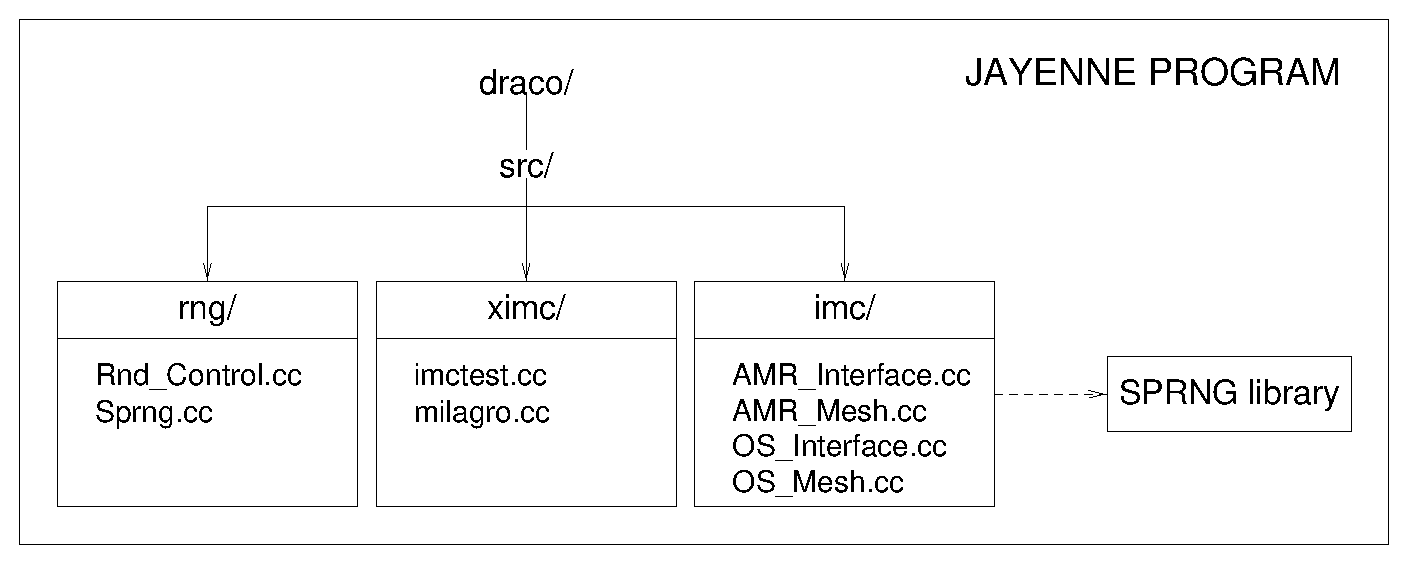
\includegraphics[width=5in]{jdir.eps}}
  \caption{\pkg{Jayenne} program structure in \draco.}
  \label{fig:Jayenne}
\end{figure}
We can show that this organization is both poorly structured and does
not conform to the \draco\ mission statement.  First, the \pkg{imc}
directory contains several interface classes.  These are not
necessarily reusable components, and, in an ideal world, these would
be provided by the host, or customer.  By placing these classes
directly in \draco\ the distinctions between the customer and the
provider are blurred.  The directory \pkg{ximc} contains stand-alone
executables.  \draco\ products are library components; executable
products should not be in \draco\footnote{An exception is executables
  for levelized component testing.}.  In fact, a stand-alone
executable is no different from a host code customer in principle.
The only difference is that the customer and supplier are both in XTM.

Finally, \pkg{Jayenne} provides random number component classes in
\pkg{rng}.  These classes are a wrapper for a vendor supplied library,
\pkg{SPRNG}.  Where is this library located?  What organizational
principles does \draco\ provide for such a library?  The answer is,
``Whatever the package developer decides.''  Thus, different vendor
libraries can be, and are, treated in many different ways in \draco.

In summary, the organizational structure for \pkg{Jayenne} is
inconsistent with the \draco\ mission statement.  First, non-reusable
interfaces (APIs) are located directly in a component directory;
second, in the \pkg{ximc} directory only executables are provided.
Finally, a set of wrapper components is provided without provision for
including the necessary external vendor library.  In addition,
this layout does not yield any information about what products will
be produced.

We can rectify the present institutional problems in \draco\ by
returning to the mission statement.  However, to do this we must first 
define a super-organizational structure that allows interfaces,
stand-alone executables, and external vendor libraries to be easily
defined in a \draco-compatible environment.  A proposed architecture
that accomplishes this stated objective is the subject of the
following sections.

%%---------------------------------------------------------------------------%%

\section{Proposed XTM Product Architecture}
\label{sec:architecture}

The superstructure of the CVS repository that will clarify the \draco\ 
issues illucidated in the preceding sections has a product-oriented
organization.  We must think of \draco\ as providing transport
components, or packages, as product deliverables.  In this section we
will develop a hypothetical code system architecture under CVS that will
promote both code development and package delivery.  

\subsection{CVS Directory Organization}

Consider the CVS repository model shown for a hypothetical code system
in Figure~\ref{fig:cvsroot}.  Let us begin our analysis of this system
by
\begin{figure}
  \centerline{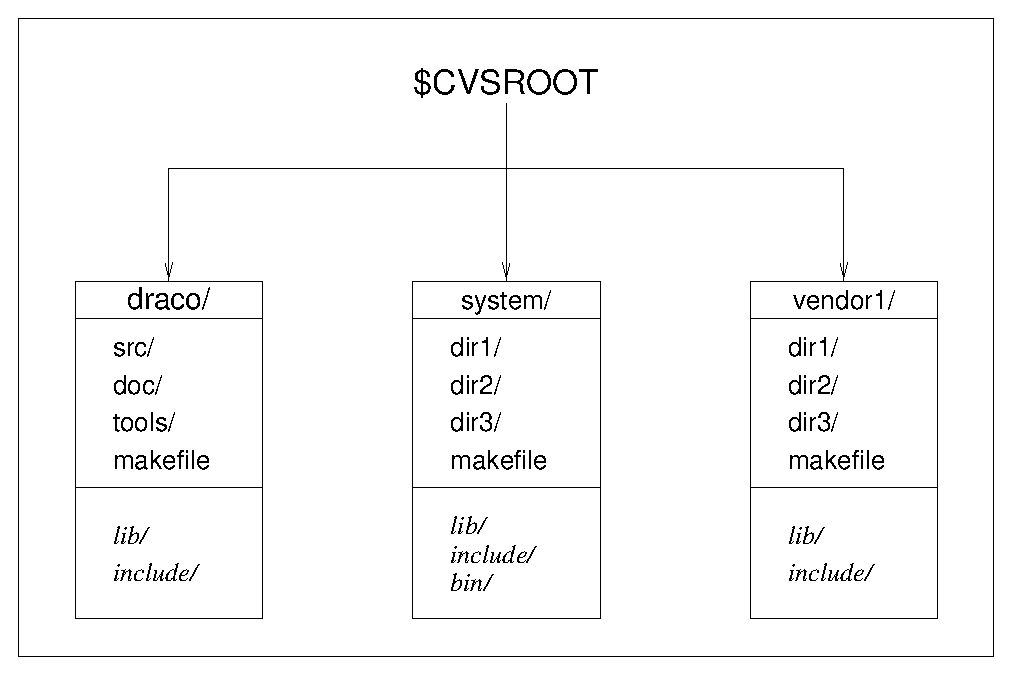
\includegraphics[width=5in]{cvsroot.eps}}
  \caption{A hypothetical code system in the XTM CVS repository.}
  \label{fig:cvsroot}
\end{figure}
clarifying the terminology that we will use throughout this report. A
\latin{product} is anything that is produced from a source code tree
\cite{ja94}.  A \latin{project} is an undertaking that has a definite
beginning and ending date and produces a product.  In our case, a
\latin{system} is a code, or group of codes, that persists over time
\cite{tn98}.  A \latin{program} is an umbrella for one or more
systems\footnote{We adopt the program concept to parallel the S-7
  practice of placing one or more common codes under an universal
  project name, ie.  Crestone, Blanca, etc.}.  A project is enacted to
add components, enhancements, or features to a system.  In the case of
the \pkg{Jayenne} program, we have a two month project to interface
\pkg{Milagro} with \pkg{Rage} that results in a new
\pkg{Product-Module} called \pkg{Milstone}.  An additional project
might be to add multigroup to \pkg{Milstone} or to refine the
interface.  However, these are each additional projects.
\pkg{Jayenne} is the program, and \pkg{Milagro} and \pkg{Milstone} are
codes, or systems, in the \pkg{Jayenne} program.

Let us return to Fig.~\ref{fig:cvsroot}.  Each system, which includes
\draco, is placed at an equivalent level in the repository.  The
essential point is that each directory should contain its own
\pkg{makefile} and directory structure.  All that is required of each
component's build system is that libraries and include files get
placed into \dir{lib} and \dir{include} directories.  This facilitates
the following features:
\begin{itemize}
\item Each directory can maintain its own build model, which is
  especially important for third-party vendor software;
\item When checking out product-modules, a master makefile can easily
  control each component directory by calling that directory's
  \pkg{makefile};
\item The products supplied by each system are easily recognizable in
  the \dir{lib} and \dir{bin} directories.
\end{itemize}
An exception is the \dir{system} directory.  The difference is that
the \pkg{System} may produce executables instead of, or in addition
to, libraries as its product.  We will illucidate this point in the
following sections.

Let us describe in detail each component directory in the CVS
hierarchy.
\begin{itemize}
\item \dir{\pkg{System}}.  This directory contains the final product.
  The \pkg{System} product is a set of library components, an
  executable, or both.  Interfaces to host codes and stand-alone input
  decks belong in this directory.  In addition, classes and code
  modules that are unique to a particular product belong here.
\item \dir{\draco}.  This directory contains components that are used
  by the \pkg{System}.  In computer-science parlance, the classes in
  \draco\ are generic base components that require template classes
  for use. The products of \draco\ are either archive (.a) or shared
  (.o) libraries.  Executables are not products of \draco.  In fact,
  the only executables in \draco\ exist for unit testing and
  regression testing \cite{la96,me97}.
\item \dir{\pkg{Vendor}}.  This directory contains third-party
  software that is used by \draco\ or the \pkg{System}.
\end{itemize}
This directory organization makes a clear distinction between \draco\
components, \pkg{Vendor} components, and \pkg{System} components.
Furthermore, all necessary software to compile \draco\ and the
\pkg{System} products exist in the CVS repository and are available
for checkout to product-modules.

\subsection{CVS Module Checkout}

We have described a CVS directory structure that properly places
emphasis on products and systems that use \draco\ as opposed to
products that are hopelessly interweaved within \draco.  We now turn
our attention to system checkouts for product development and
delivery.  The objective of product checkouts is to develop and
deliver code.  We hope to define a process by which directories in
the CVS repository are checked out as product-modules for both code
development and code delivery to customers.  In other words, given the
CVS directory structure shown in Fig.~\ref{fig:cvsroot}, what methods
are required to formulate a package for development and delivery to
customers.

A proposed product-module structure that results from CVS
checkout is shown in Fig.~\ref{fig:checkout}.
\begin{figure}
  \centerline{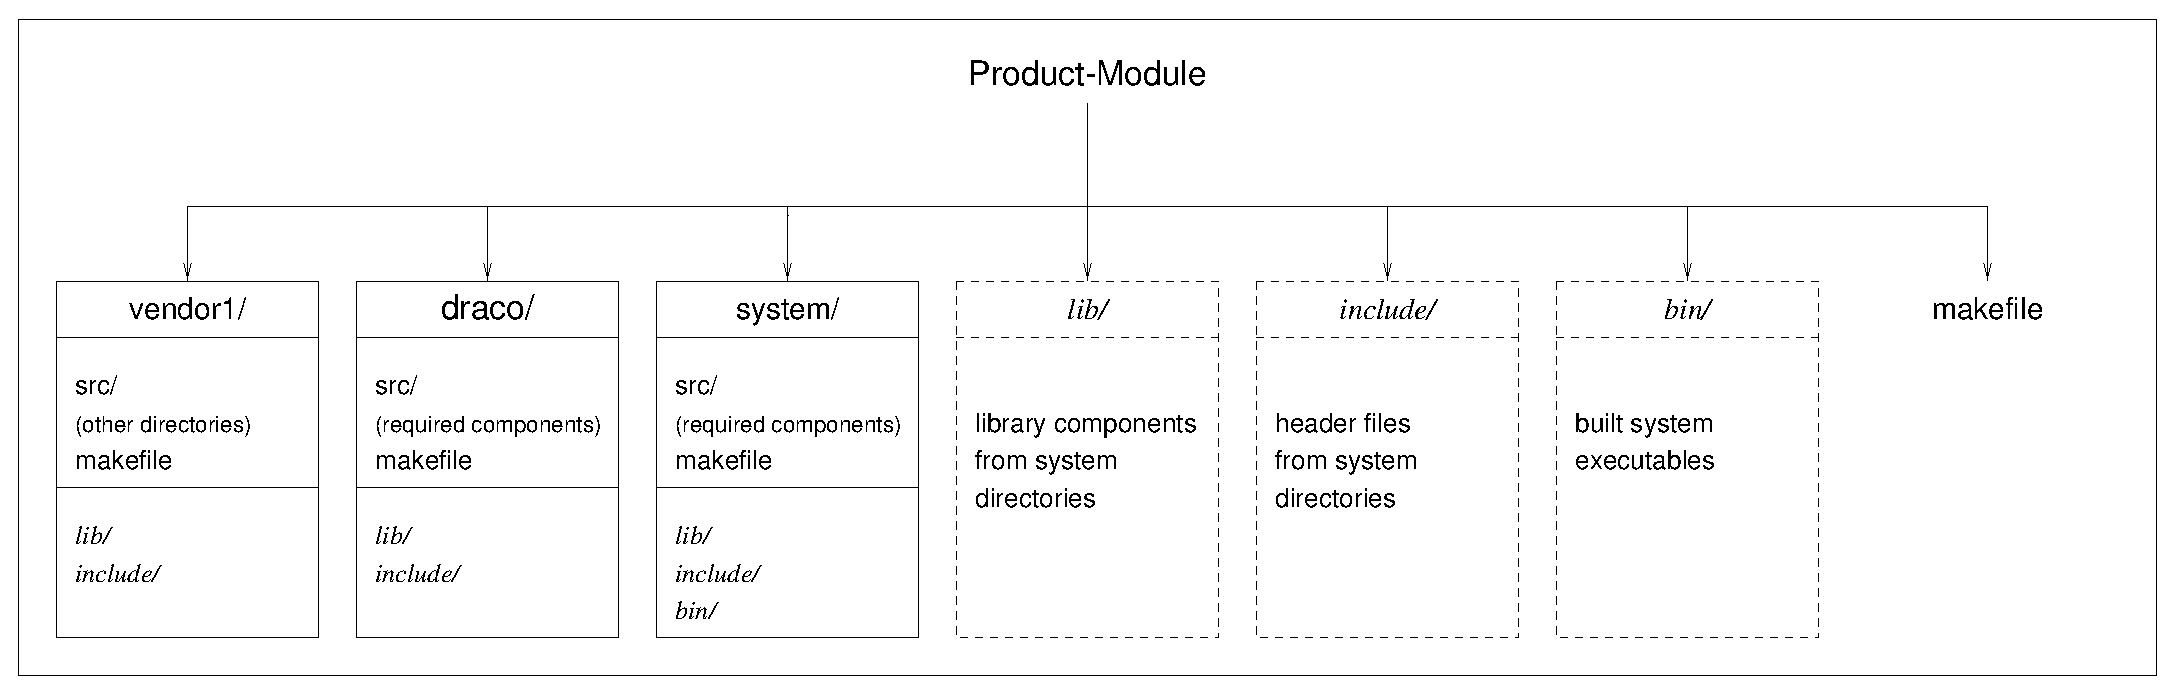
\includegraphics[width=6in]{checkout.eps}}
  \caption{Project-module organization upon CVS checkout.  Components
    in dashed-line boxes are the products produced by the system.}
  \label{fig:checkout}
\end{figure}
The \pkg{\$CVSROOT/CVSROOT/modules} file contains the definition of
the \pkg{Product-Module}.  We shall proceed to analyze this
architecture in detail.  First, notice that only the components
required to produce the products of the \pkg{Product-Module} are
included under \dir{draco} and \dir{system}.  In addition, only vendor
components required to compile the products are included in the
checkout.  Also note that the products, in dotted lines and italic
print in Fig.~\ref{fig:checkout}, can be library components,
executables, or both.

This organizational structure preserves the distinction between
\draco\ components, interfaces, vendor components, and products.
\draco\ provides the necessary package components to produce either a
stand-alone executable or a package for a host-code.  The components
in \draco\ make no distinction between the two.  Both interfaces to
host-codes and interfaces to a stand-alone executable are parts of the
\pkg{System}.  That is the advantage and the purpose of the generic
programming architecture in \draco.  The end product of the
\pkg{Product-Module} is either the library components in \dir{lib},
executables in \dir{bin}, or combinations of both.

A master \pkg{makefile} compiles the components in
\pkg{System}-dependent components in \dir{draco}, \dir{system}, and
\dir{vendor}.  These products are then placed in the appropriate
\dir{lib} and \dir{bin} directories.  In this form, our products can
be delivered to ASCI code teams for simple incorporation into large
host codes, or the \pkg{Product-Module} can stand-alone if the product 
is an executable program.

%%---------------------------------------------------------------------------%%

\section{Product Development Responsibilities}
\label{sec:response}

Having formulated a new organizational architecture for product
development within XTM, we must define responsibilities for different
members of the code development community.  Let us return to the CVS
organizational structure in Fig.~\ref{fig:cvsroot}.  The primary
components for the transport package reside in \draco.  These
component libraries are the exclusive responsibility of XTM code
product teams.  Let us summarize what these responsibilities entail:
\begin{itemize}
\item \draco\ consists of component libraries exclusively, the only
  executables in \draco\ are used for levelized component
  verification and testing;
\item CVS checkout of \draco\ components is restricted to XTM code
  product teams; modifications to these components should not be
  made by external parties;
\item code and design reviews of \draco\ components are the
  responsibility of XTM \draco\ system developers;
\item verification of \draco\ components are the responsibility of
  XTM \draco\ system developers.
\end{itemize}
This list clearly defines the responsibilities of \draco\ team
members.

Returning to Fig.~\ref{fig:cvsroot}, we must clarify some issues
between the \dir{vendor} and \dir{system} directories.  First, the
\pkg{Vendor} components are {\bf always} supplied by a third party.
Examples of \pkg{Vendor} components are \pkg{Metis} and \pkg{Sprng}.
The \pkg{System} components, which are the final products, may
be supplied by XCI, XTM, a third party, or by a combination of these
elements.  For example, the interface to a \draco\ transport package
resides in the \dir{system} directory.  At present, product
development teams in XTM supply these components.  In the future, XCI
should provide them.

With these clarifications in mind, the responsibilities of XTM
\latin{vis-a-vis} \pkg{Vendor} packages are:
\begin{itemize}
\item \pkg{Vendor} components are checked into the CVS repository as
  released versions, CVS checkouts for development are not allowed;
\item \pkg{Vendor} component upkeep is the responsibility of the
  provider, not XTM.
\end{itemize}
In essence, a \pkg{Vendor} supplied package is placed into the XTM
repository in an usable state.  No upkeep, other than acquiring new
releases, is required by XTM code-product teams.

The responsibilities of \pkg{System} component providers may be more
complicated because several parties may have responsibility for
certain parts of the code.  The general responsibilities of a
\pkg{System} interface developer are:
\begin{itemize}
\item \pkg{System} components provided by external parties (XCI, etc.)
  are checked into the repository as released versions, version
  control and maintainence are the responsibility of the component
  developers, not XTM;
\item \pkg{System} components developed by XTM code product teams are
  maintained and updated through CVS checkout;
\item \pkg{System} component code and design reviews are the
  responsibility of both XTM and the providers of the components;
\item \pkg{System} product verification is the responsibility of both
  XTM and the providers of the component products.
\end{itemize}
As opposed to external vendor products, many aspects of \pkg{System}
components are under the pervue of both XTM and the component
developers.  In many cases, such as stand-alone executables, XTM is
both the customer and developer of these systems.

Let us recap the essential guidelines for XTM with regards to code
checkout in the CVS repository.  First and foremost, no external
parties should checkout code from the XTM CVS repository.  External
development teams providing either \pkg{vendor} or \pkg{System}
components deliver released versions to XTM.  XTM is responsible for
checking these versions into our repository.  XTM is not responsible
for upkeep of these components.  This guideline parallels the method
by which XTM components are handled by XCI and other customers.  We
deliver released versions of components to XCI for use in their codes.
From XCI's perspective, they are not responsible for upkeep or
revision control of these packages.

%%---------------------------------------------------------------------------%%

\section{Product Documentation}
\label{sec:document}

Documentation has been a weak point in the \draco\ program.  Most
components have no, or poor, documentation. Every product in XTM
should maintain the following baseline documentation:
\begin{itemize}
\item product layout;
\item product user manuals.
\end{itemize}
The product layout documents defines what \draco, \pkg{Vendor},
and \pkg{System} components make up the product.  Also, this document
defines the product.  Product user manuals describe how the product
is used.  These documents should be archived in the CVS repository as
described below.

In addition to the baseline requirement, each component in the product
source tree should have documentation.  Documentation, both initial
compilation and updates, is the responsibility of the code developer.
Documents pertaining to code components should be stored in the CVS
repository as illustrated in Fig.~\ref{fig:doc}.  Documents that
\begin{figure}
  \centerline{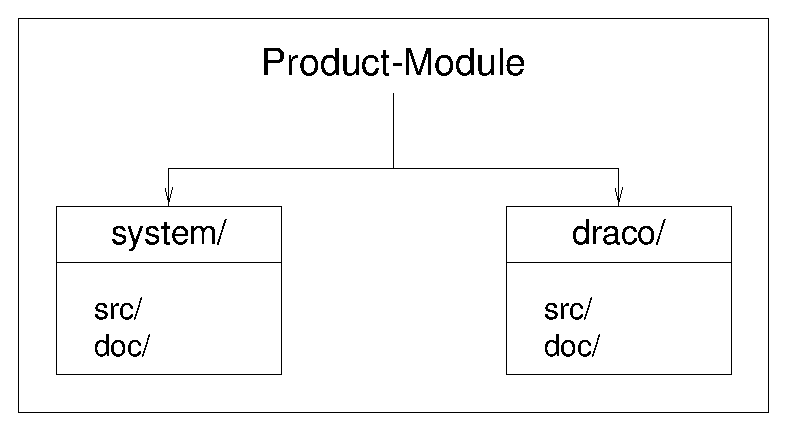
\includegraphics[width=4in]{doc.eps}}
  \caption{Document archiving in XTM product-modules.}
  \label{fig:doc}
\end{figure}
belong in the CVS repository under the code source trees should
adhere to the following topics:
\begin{itemize}
\item code design documents;
\item code methods documents;
\item code performance documents.
\end{itemize}
In fact, nearly any documentation that stresses the code package may
be put in the code source tree.  Documents that do not describe any
specific code features do not belong in the source tree.  For example, 
a paper describing the $P_{1}$ transport methods used and implemented
in \pkg{Solon} should be archived in the \pkg{Solon} directory.  A
paper about $P_{1}$ transport methods, without reference to the
methods used in \pkg{Solon}, belongs elsewhere.

Documentation should  be placed under the appropriate directory in 
the CVS source tree.  For example, \draco\ components should be
documented in \draco.  \pkg{System} components should be documented
under the \dir{system} directory.

%%---------------------------------------------------------------------------%%

\section{Sample Product Layout}

We will illustrate the concepts set forth in
Secs.~\ref{sec:architecture}, \ref{sec:response}, and
\ref{sec:document} with an example.  The \pkg{Milagro} IMC package
will serve as our demonstration package.  \pkg{Milagro} is a
stand-alone IMC package that is built within \draco\ and uses an
external vendor package, \pkg{SPRNG}.  Figure~\ref{fig:milagro_co}
shows the product-module, \pkg{Milagro}, that results from CVS
checkout.
\begin{figure}
  \centerline{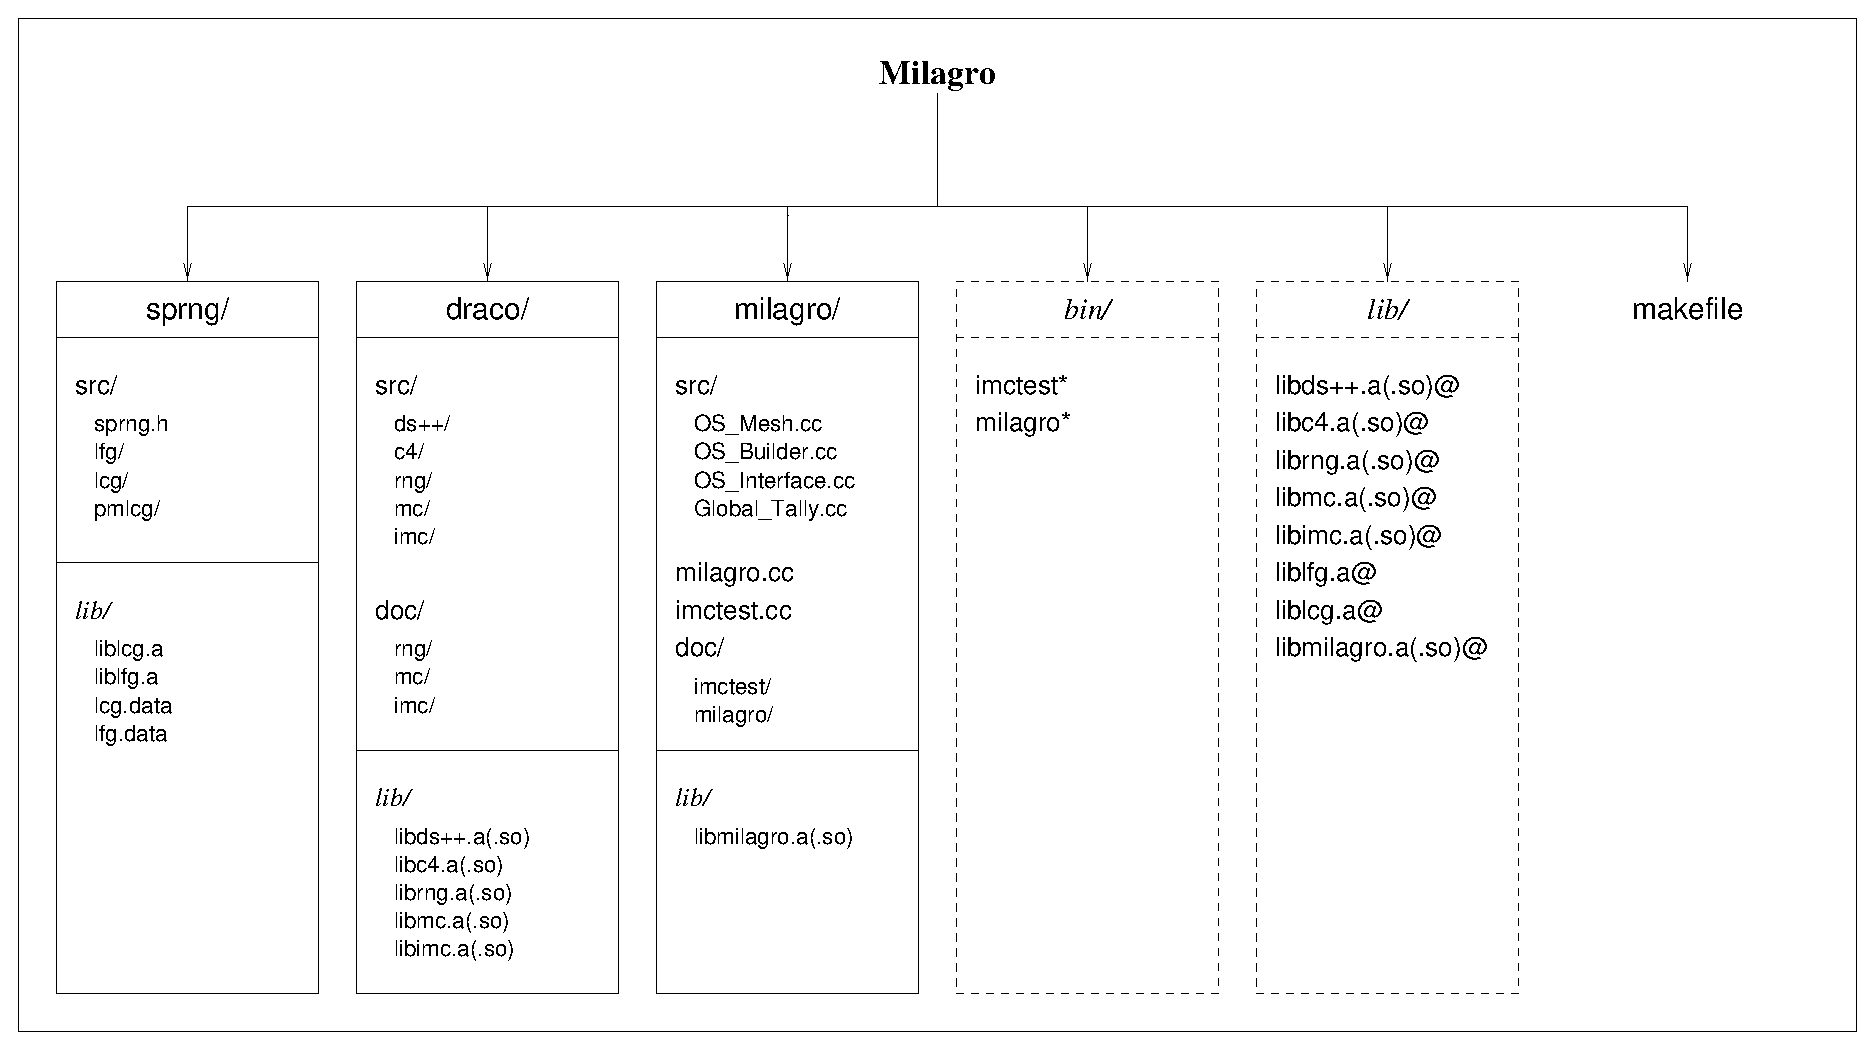
\includegraphics[width=6in]{milagro_co.eps}}
  \caption{Project-module organization of \pkg{Milagro} upon CVS
    checkout.  Components in dashed-line boxes are the products
    produced by the top-level \pkg{Milagro} \dir{makefile}.}
  \label{fig:milagro_co}
\end{figure}
This example illustrates the CVS organization postulated in
Fig.~\ref{fig:checkout}. 

Figure~\ref{fig:milagro_cvs} shows the \pkg{Milagro} components in the 
CVS repository.  This example illustrates the general CVS organization 
\begin{figure}
  \centerline{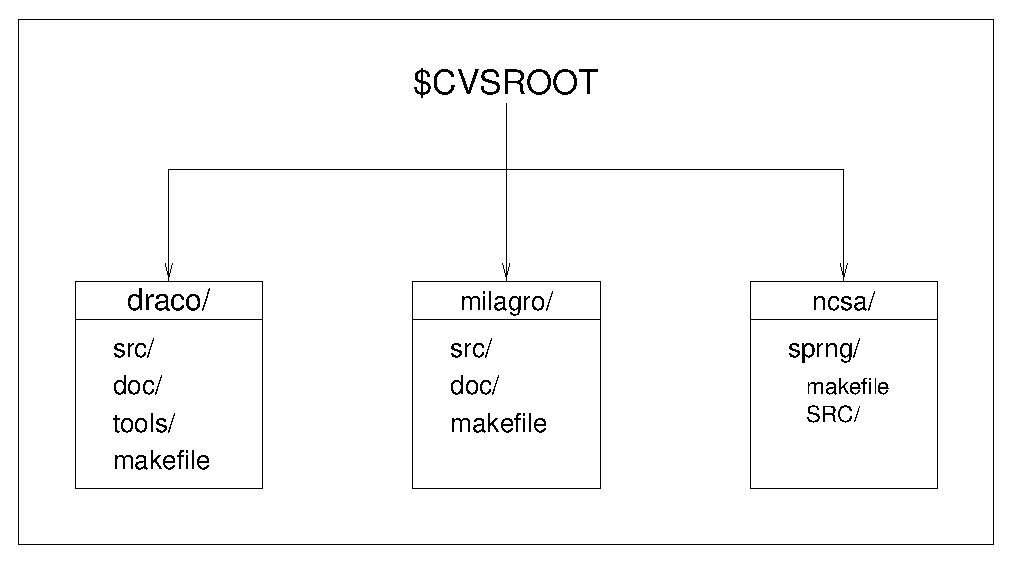
\includegraphics[width=5in]{milagro_cvs.eps}}
  \caption{The \pkg{Milagro} module components in the CVS repository.}
  \label{fig:milagro_cvs}
\end{figure}
shown in Fig.~\ref{fig:cvsroot}.  Figure~\ref{fig:milagro_cvs} clearly 
illustrates the relationship between unique, product-specific files,
vendor-supplied libraries, and reusable, generic \draco\ components.

An additional option to the checkout plans illustrated in
Fig.~\ref{fig:checkout} and \ref{fig:milagro_co} is to define a
\dir{makefile} variable \$draco\_root.  Thus, if a compiled version of
\draco\ existed somewhere in the system, only the \pkg{Product-Module}
directories would be required to compile the product libraries and/or
executables.  However, we note that this plan is more for deliverables
to customers; it is not optimal for XTM code development.

%%---------------------------------------------------------------------------%%

\section{Additional Topics}

There are many issues that require formal documentation for this plan
to be implemented in a proper way.  Some of these issues have been
mentioned above; however, many have not.  XTM should endeavor to
develop a set of \latin{primers}, such as this one, with formal lab
document numbers.  These can be compiled into a reference manual for
future transport code development.  Topics that require
\latin{primers} are:
\begin{itemize}
\item {\em Setting Up a Product-Module in the CVS Repository.}
\item {\em Product Releases in XTM.}
\item {\em The \draco\ Build System.}
\item {\em DegaGnu and Regression Testing in \draco.}
\item {\em \pkg{Vendor} Libraries Used in \draco.}
\item {\em Code Reviews in XTM.}
\item {\em Bug Tracking in \draco.}
\item {\em Design-by-Contract$^{\text{\scriptsize\textsl{TM}}}$
    Verification in \draco.}
\item {\em Project Reporting in \draco\ and XTM.}
\end{itemize}
This list is not exhaustive; however, it is a good start for
developing a comprehensive list of references for XTM code developers.

%%---------------------------------------------------------------------------%%

\section{Summary}

In the preceding sections we set out to address three issues:
categorizing the deficiencies in \draco\ and XTM's \latin{modus
  operandi} at present, proposing a new code development architecture
that places the proper emphasis on products and makes distinctions
between components and interfaces, and, finally, proposing new
guidelines for working with \draco\ in this new environment.  Our
proposed reorganization and guidelines have been aimed at creating
``inherently manageable'' projects within XTM.  To achieve that goal,
our code systems must have organizational principles that allow one to
design and implement new code without having to stop at each step to
view the big picture.  The code-development architecture espoused in
this note makes these projects self-manageable.

We have also touched upon other issues, most notably documentation.
We hope to develop a set of \latin{primers} that will illustrate the
mechanics needed to design \pkg{Product-Modules} that use \draco.  Our 
objective is to ``automate'' this process as much as possible so that
XTM code teams can spend more time developing methods and algorithms
and less time working on large-scale code infrastructure.

%%---------------------------------------------------------------------------%%

\section{Acknowledgments}

This document is the result of in-depth discussions with XTM \draco\
team members Todd Urbatsch, John McGhee, Mark Gray, Randy Roberts,
and Shawn Pautz.  Also, we acknowledge former XTM team member Geoff
Furnish who provided the concept \draco.

%%---------------------------------------------------------------------------%%

\bibliographystyle{../tex/rnote}
\bibliography{../bib/draco}

\closing
\end{document}

%%---------------------------------------------------------------------------%%
%% end of rn98046.tex
%%---------------------------------------------------------------------------%%
